\subsection{\cinterface}
\label{sec:client_interface}

The \aclient[] interface is illustrated in figure \ref{fig:client_interface}.
After login, the \aclient[] is presented with the \textit{main} window. 


\begin{figure}[p]
	\centering
		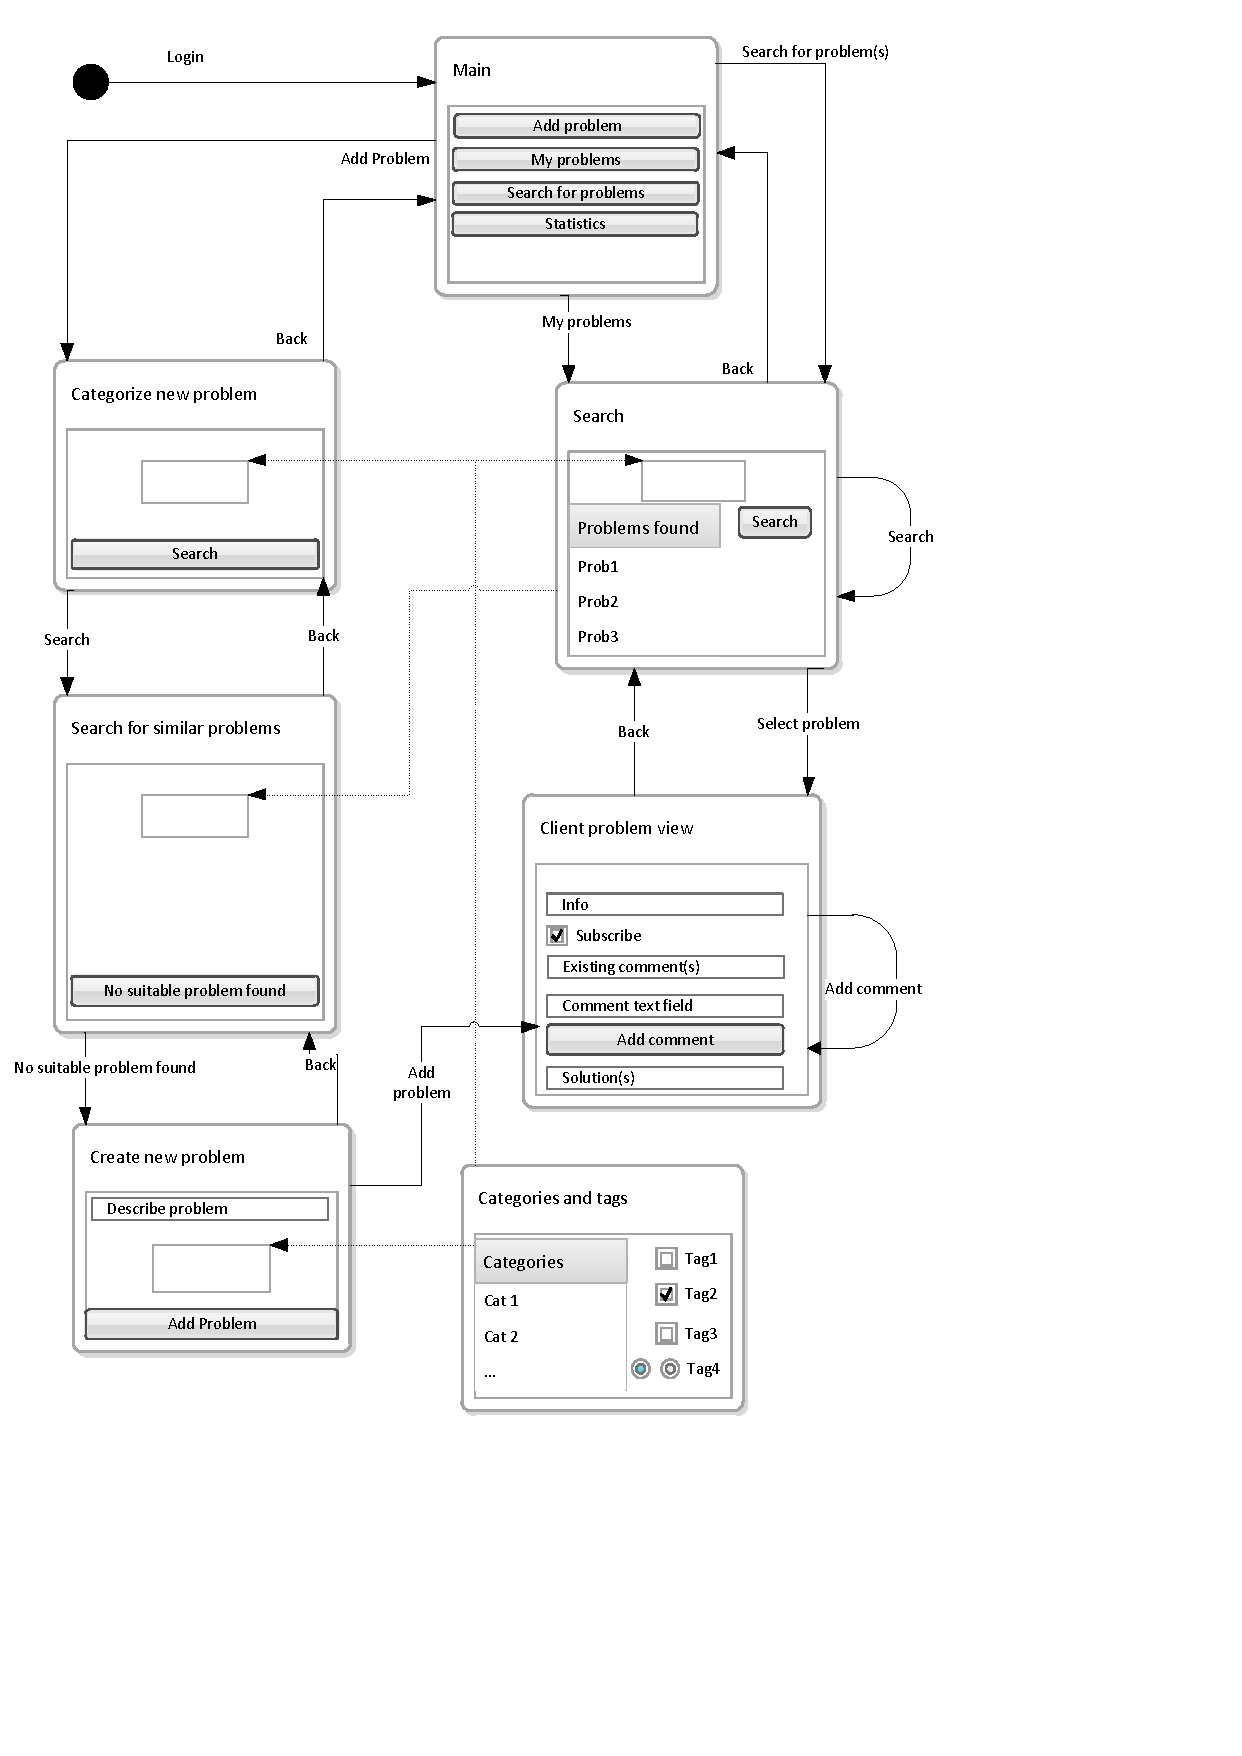
\includegraphics[width = \textwidth, clip=true, trim=0 4cm 5cm 0]{input/application_domain_analysis/Navigation_DiagramClient.pdf}
	\morscaption{Navigation diagram of the client interface}
	\label{fig:client_interface} %fig:Navigation_DiagramAdmin
\end{figure}

\subsubsection{Main}
The \aclient s main window allows the \aclient[] to choose what to do in the helpdesk system. The ``Main'' window have three buttons:
\begin{itemize}
	\item The ``Commit Problem'' button which sends the user to the ``Categorize new problem'' window.
	\item The ``My problems'' button which sends the user to ``Search'' window.
	\item The ``Search for problems'' button which sends the user to ``Search'' window.
\end{itemize}

%The \aclient[] main window have three buttons: ``Add problem'', ``My problems'' and ``Search for problems''.
%The ``Add problem'' button sends the user to the ``Categorize new problem'' window.
%The ``My problems'' and ``Search for problems'' button sends the user to ``Search'' window.

\subsubsection{Search}
The search windows is used to search for problems containing specific tags or problems posted by the client self. The ``Search'' window contains the following elements:
\begin{itemize}
	\item The ``Categories and tags'' frame, see paragraph below.
	\item A settings panel.
	\item A search button that triggers the search, see paragraph below.
	\item A list containing the problems matching the settings and tags.
\end{itemize}
A problem can be double clicked to view details about the problem in the ``Client problem view'' windows.
%The search window contains a search button, a list where found problems are displayed, a settings and the frame ``Categories and tags''
%The search button will start a search with the current configuration and show the results in the list. 

\paragraph{Settings}
The ``Settings'' frame contains configurations options for the search.
The frame contains the following elements:
\begin{itemize}
	\item My problems 
	\item Unsolved problems
	\item Solved problems 
	\item Number of search results
\end{itemize}
When a search is preformed these options are checked and they will effect the result of the search.

\paragraph{Categories and tags} 
This frame is used in a few other windows as well. 
The frame contains:
\begin{itemize}
	\item A list of categories and the tags attached to it. 
	\item A checkbox for each tag.
\end{itemize} 

\subsubsection{Client Problem View}
This window contains information about the selected problem. The window contains the following:
\begin{itemize}
	\item A info field which contains relevant information about the problem e.g. the description of the problem.
	\item A subscription check-box, clients subscribed to the problem will receive notifications when then problem changes. 
	\item A text field with all the previous entered comments if any.
	\item A field to write new comments in.
	\item The button ``Submit comment'' which submits the comment.
	\item A field with non or more solutions written by the staff members.  
\end{itemize}


%There is , , a text field with all the previous entered comments if any, a field to write new comments in, a button called ``Add comment'' to submit the new comment and a field with non or more solutions written by the staff members.  

\subsubsection{Categorize New Problem}
To add a new problem the \aclient[] need to select the tags which best describes the problem. The window contains the following elements:
\begin{itemize}
	\item The frame ``Categories and tags''.
	\item The button ``Search for this kind of problems'' which sends the \aclient[] to the window ``Search for similar problems''
\end{itemize}
%This window contains  and a search button. When a search is conducted the window ``Search for similar problems'' is opened. 

\subsubsection{Search for Similar Problems}
A search is preformed with the selected tags from the previous window, a list with similar problems are displayed. This window includes the following: 
\begin{itemize}
	\item The window ``Search'' with all the the search property.
	\item A button called ``No problem suffice'' which loads the window ``Create new problem''.
\end{itemize}
The found problems can be  clicked and the user is redirected to  the window ``Client problem view''. 

\subsubsection{Create new problem}
The ``Create new problem'' window's purpose is to describe, categorize, suggest deadline and submit the problem. The window contains the following elements:
\begin{itemize}
	\item A text field where information about the problem can be entered.
	\item The frame ``Categories and tags'' enables the \aclient[] to change and add tags so the problem is best describe.
	\item A calendar where a deadline can be suggested to the \astaff[] member.
	\item ``Create'' submits the problem and send the user to the ``Client problem view''.
\end{itemize}

%The frame ``Categories and tags'' enables the \aclient to pick what tags describe the problem best, the . When the ``Add problem'' is pressed the problem is send and the user is directed to the ``Client problem view'' where he can see the final description of the problem and relevant statistics.    






